%-----------------------------------------------------------------------------%
\chapter{METODE PENELITIAN}
%-----------------------------------------------------------------------------%

%
\vspace{4.5pt}

\section{Permasalahan pada Software Deployment}
Dimasa saat ini dimana sebuah permintaan pasar pada sektor teknologi berubah cepat dan digunakan oleh banyak orang. Diperlukan juga cara mendeliver  teknologi tersebut secara cepat, aman, dan reliable.
Dengan adanya permintaan yang cukup banyak dan berubah ubah setiap saat.
Banyak perusahaan yang menerapkan metode agile development pada pengembangan produk nya.
Pada sistem agile biasanya suatu masalah dipecah menjadi sebuah stories dan dilakukan  estimasi effort oleh developer untuk menyelesaikannya.
Banyak juga manager yang  mengukurnya ketika sebuah stories selesai itu terdapat pikiran jika team nya
meningkat dalam hal kecepatan (velocity) development. Dengan menggunakan  metrik velocity tersebut untuk mengukur sebuah produktifitas sebuah team  menjadikan itu bagian hal yang tidak absolute.
Apakah setiap team yang  “menyelesaikan” banyak stories dapat dibilang produktif dari segi feedback yang  didapatkan ketika produk/kode nya berjalan pada produksi ?.
\par
Menurut Forsgen pada bukunya ``Accelerate: The Science of DevOps" \cite{Forsgen2018} secara tradisional reliability diukur ketika waktu sistem tersebut  gagal.
Tetapi pada software product atau services yang modern yang selalu berganti  ganti dan kompleks, kegagalan tidak dapat dihindari lagi.
Pada bukunya juga dia  melakukan survey yang diambil pada taun 2014-2016 yang saya simpulkan secara  garis besar bahwa perusahaan
yang menerapkan observability terhadap sistem nya  mendapatkan failure rate yang sangat rendah dibanding dengan yang lainnya.

\vspace{0.5cm}
\section{Continous Delivery Meningkatkan Software Delivery Performance}
Menurut Forsgen \cite{Forsgen2018} terdapat dampak penerapan continuous delivery pada perusahaan yaitu:
\begin{enumerate}[label=\alph*.]
    \item Sebuah team dapat melakukan deployment ke tangan user secara langsung dengan cepat.
    \item Mendapatkan feedback cepat dalam kualitas software.
    \item Meningkatkan produktifikasi developer.
\end{enumerate}
\vspace{0.5cm}
\subsection{Metode Continuous Delivery (CDE)}
Continuous Delivery (CDE) adalah disiplin dalam rekayasa perangkat lunak dimana sebuah team dapat memproduksi
perangkat lunak yang valuable secara incremental dalam siklus yang pendek dan menjamin sebuah perangkat lunak dapat di-release pada waktu kapan saja \cite{Chen2015b}.
\begin{figure}[h]
    \centering
    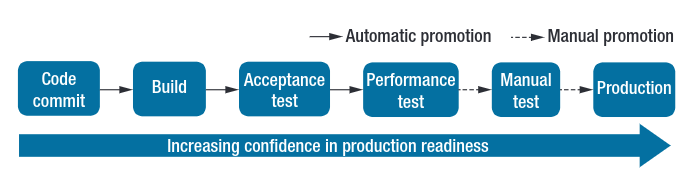
\includegraphics[width=1\textwidth]{figures/continouse-delivery-pipeline.png}
    \caption{Contoh pipeline dalam Continous Delivery}
\end{figure}

\subsection{Metode Continuous Deployment}
Perbedaan mendasar dari Continuous Delivery (CDE) dan Continuous Deployment (CD) adalah dimana implementasi semua fase
dilakukan secara automatis tanpa memerlukan intervensi manusia, deployment
ke tahap environment produksi juga bisa dilakukan secara automatis, tetapi biasanya memerlukan intervensi pada satu tahap \cite{Ramadoni2021}.
\vspace{0.5cm}
\section{Deployment Pada Kubernetes}
Pada padasarnya terdapat 2 metode yang digunakan untuk melakukan
deployment pada sebuah aplikasi pada kubernetes yaitu pull method dan push method \cite{Ramadoni2021}.
Perbedaan mendasar dari pull method dan push method terdapat pada agent yang melakukan
deployment \cite{GitOps}. Pada push method sebuah agent melakukan deployment sebuah service terhadap suatu platform (eg, kubernetes).

\subsection{Literatur Pull-based Deployment}
Berdasarkan penelitian terbaru, pendekatan pull-based deployment telah terbukti memberikan beberapa keunggulan signifikan dalam konteks GitOps \cite{Korhonen2021}. Beberapa keunggulan utama dari pull-based deployment antara lain:
\begin{enumerate}
    \item \textbf{Keamanan yang Lebih Baik}: Tidak memerlukan kredensial akses eksternal ke cluster Kubernetes, sehingga mengurangi risiko kebocoran kredensial.
    \item \textbf{State yang Konsisten}: Operator secara berkala memeriksa dan menyinkronkan state yang diinginkan dengan state aktual di cluster.
    \item \textbf{Recovery Otomatis}: Dapat secara otomatis mengembalikan konfigurasi ke state yang diinginkan jika terjadi perubahan yang tidak diinginkan.
    \item \textbf{Multi-cluster Management}: Memudahkan pengelolaan beberapa cluster Kubernetes sekaligus dari satu sumber kebenaran.
\end{enumerate}

Menurut \cite{Sharma2022}, implementasi pull-based deployment dengan Argo CD telah menunjukkan peningkatan keandalan deployment sebesar 40\% dibandingkan dengan pendekatan push-based tradisional.
\vspace{0.5cm}
\subsection{Push-based Deployment}
Push-based deployment \cite{GitOps} merupakan strategy yang popular yang diimplementasikan oleh
tools seperti Jenkins, CircleCI, atau TravisCI.
Sourcecode dari sebuah aplikasi terdapat pada repository yang sama dengan konfigurasi YAML Kubernetes yang diperlukan untuk melakukan deployment aplikasi tersebut.
Kapan pun code dari aplikasi tersebut diupdat, pipeline akan berjalan, dimana akan membuat container image yang diperlukan.
Perlu diperhatikan juga bahwa biasanya credential environment untuk melakukan deployment pada metode Push-based. Jadi pada pipeline tersebut kita dapat melihat
configurasi rahasia yang mungkin saja terlihat oleh orang lain.
\begin{figure}[ht]
    \centering
    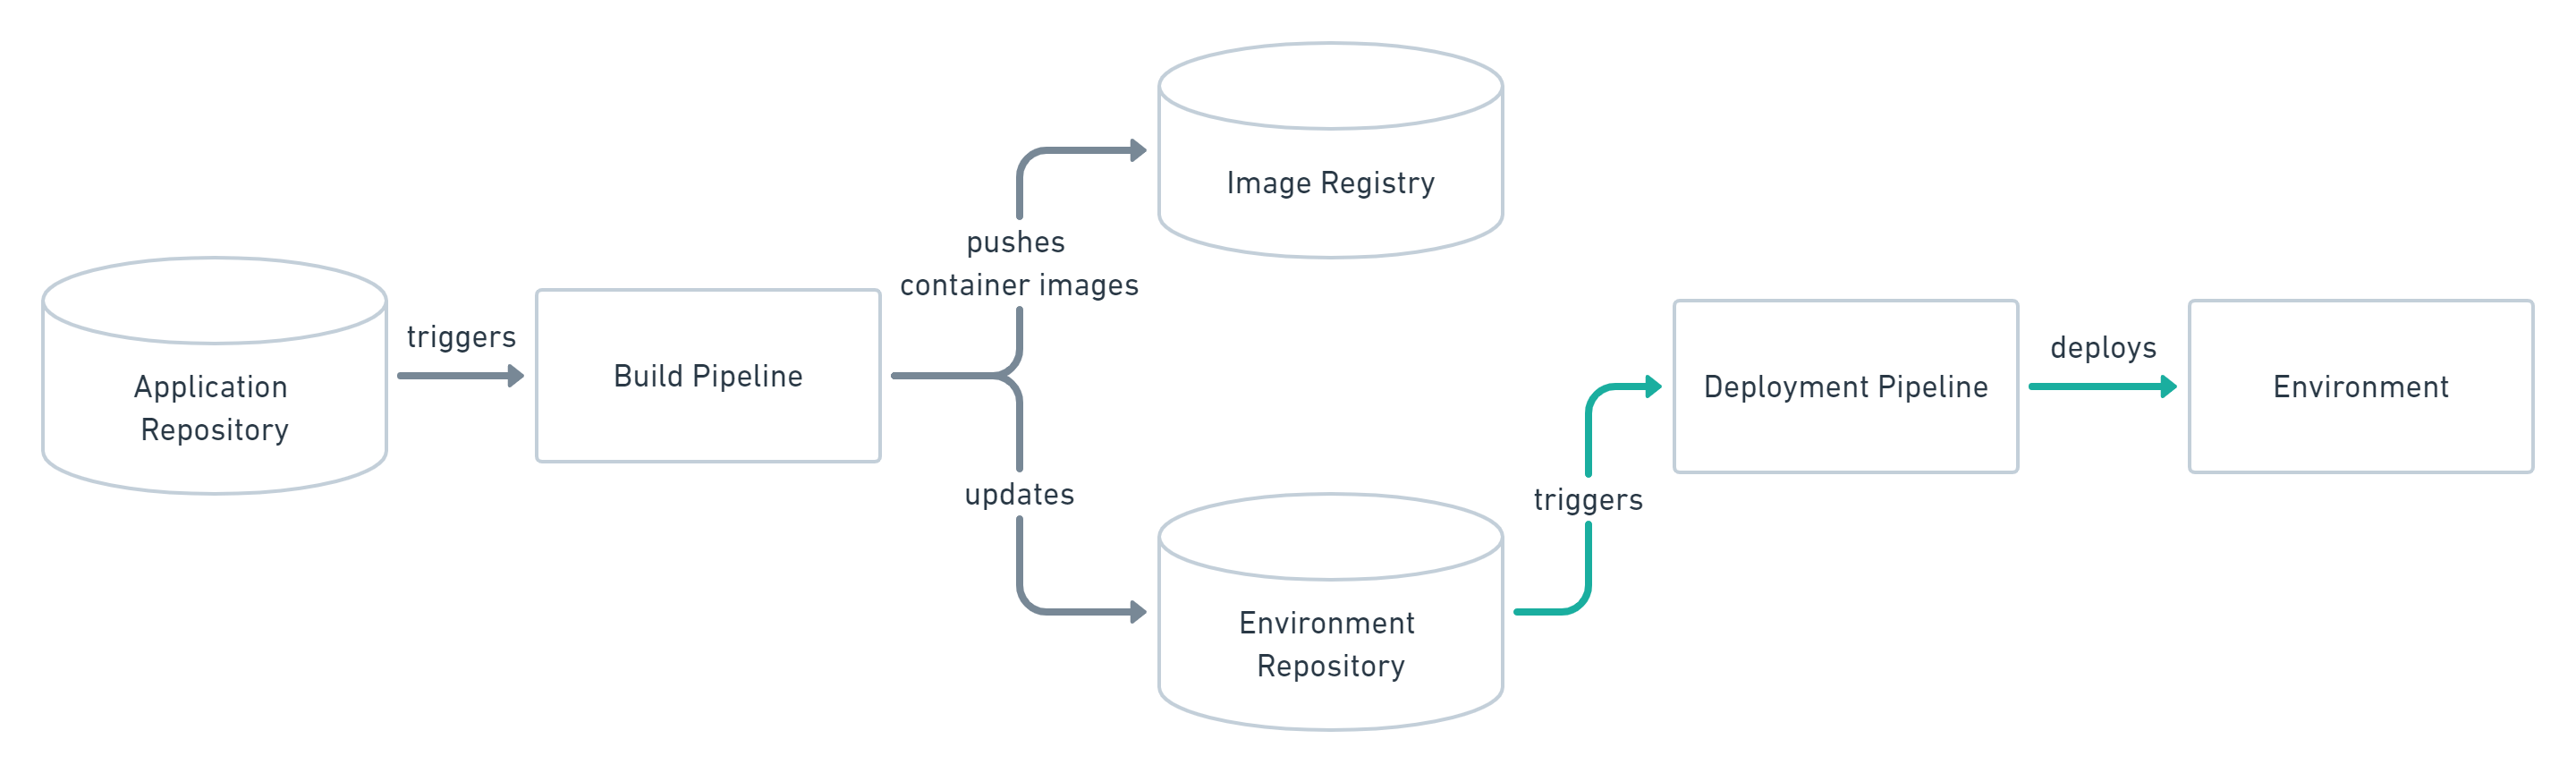
\includegraphics[width=1\textwidth]{figures/push-based.png}
    \caption{Contoh pipeline dalam push-based deployment}
\end{figure}
\newpage
\vspace{0.5cm}
\subsection{Pull-based Deployment}
Pada website insert gitops Strategi Pull-based deployment menggunakan konsep
yang sama dengan push-based tetapi berbeda pada bagaimana cara kerja pada pipeline deployment.
Secara traditional pipeline CI/CD akan di-trigger oleh event eksternal, contohnya ketika ada update kode
baru yang pada repository. Dengan metode pull-based deployment, dikenalkan sebuah operator.
Operator tersebut secara kontinu dengan interval yang dapat diatur sendiri melakukan komparasi
terhadap state yang ada di repository dengan state yang ter-deploy pada infrastructure.
Ketika terdapat perbedaan, operator melakukan update pada infrastructure untuk mencocokan state dengan apa yang ada di repository.
Operator harus berada pada environment atau kluster yang sama dengan applikasi yang akan dideploy. Dengan ini pull-based method
tidak perlu mengetahui environment eksternal karena semua sudah ada pada kluster yang sama.
\begin{figure}[h]
    \centering
    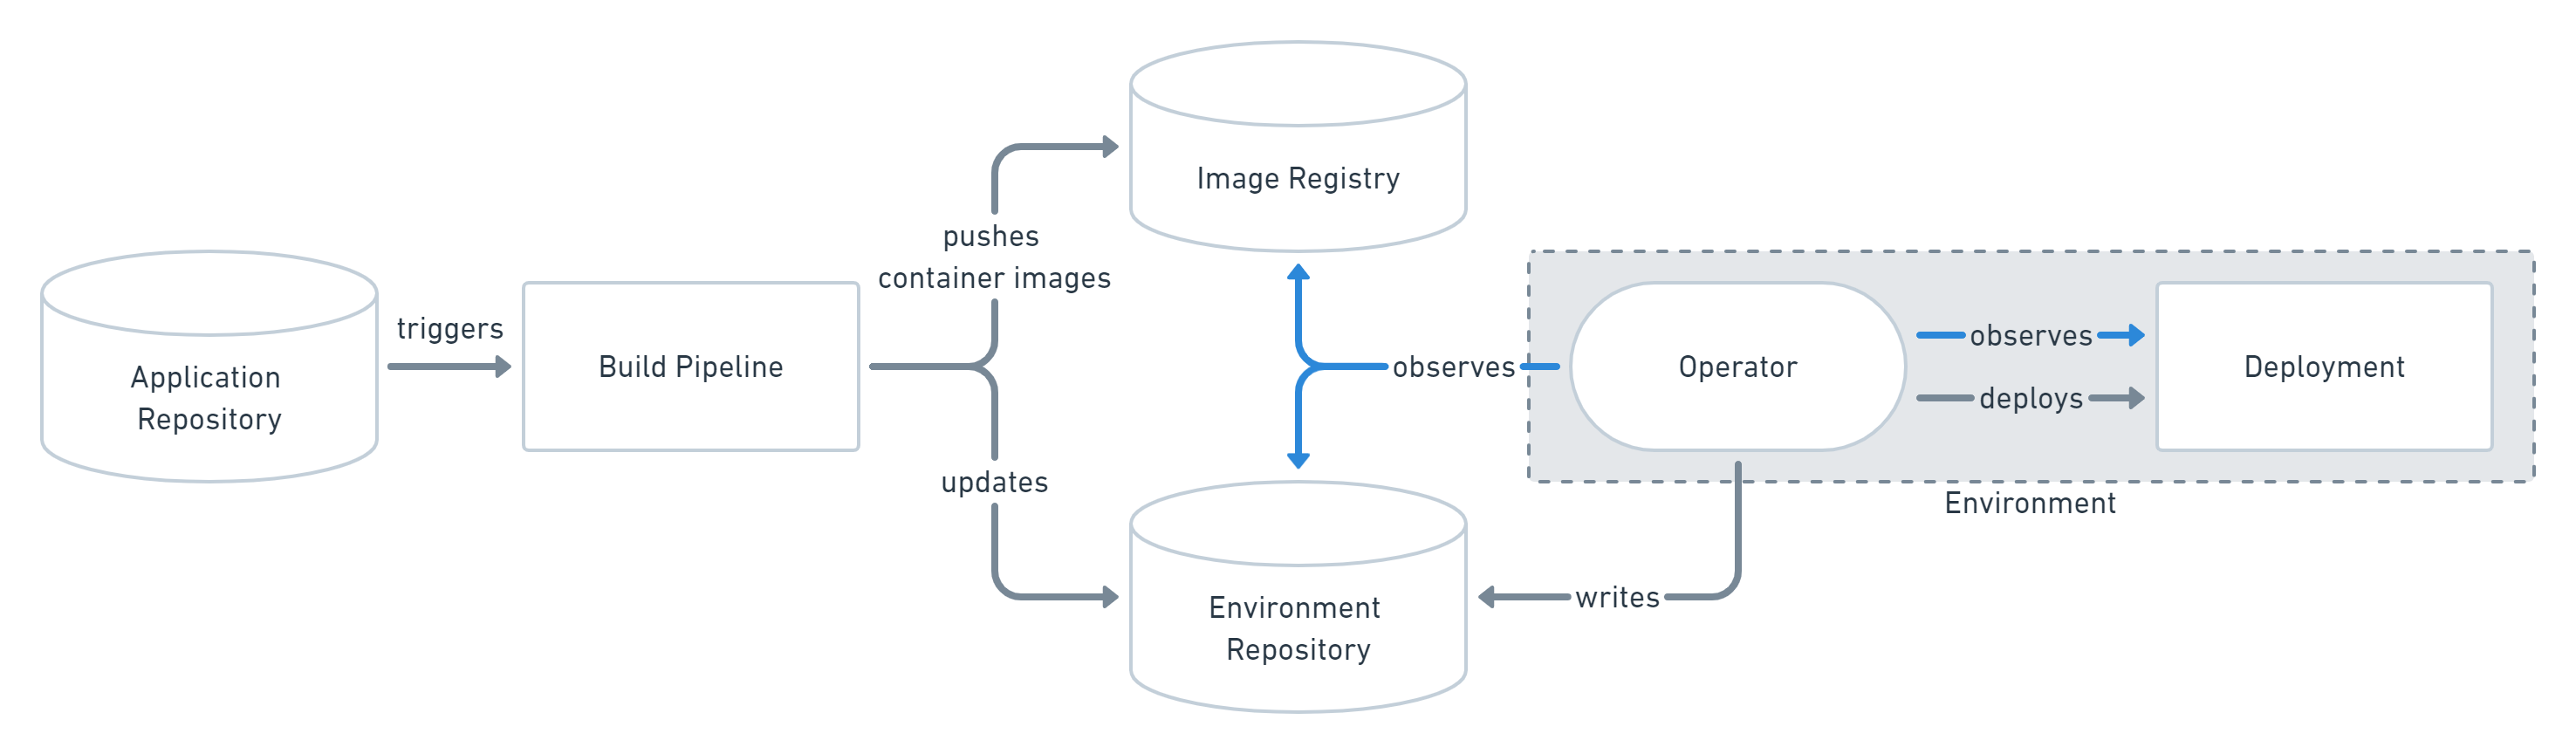
\includegraphics[width=1\textwidth]{figures/pull-based.png}
    \caption{Contoh pipeline dalam pull-based deployment}
\end{figure}
\vspace{0.5cm}

\newpage
\section{Alur Penelitian dan Implementasi}
Penelitian ini akan mengikuti alur metodologi yang terstruktur untuk memastikan pencapaian tujuan penelitian. Berikut adalah bagan alur penelitian yang akan diimplementasikan:

\begin{figure}[h]
    \centering
    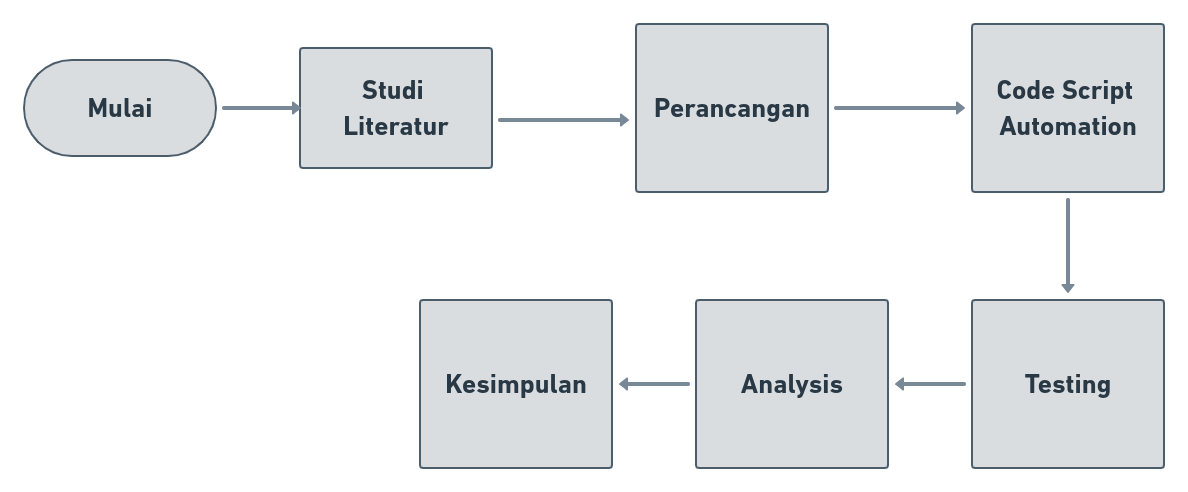
\includegraphics[width=0.9\textwidth]{figures/Tahapan Skripsi.png}
    \caption{Alur Penelitian dan Implementasi}
    \label{fig:alur_penelitian}
\end{figure}

Adapun penjelasan rinci dari setiap tahapan adalah sebagai berikut:
\begin{enumerate}
    \item \textbf{Studi Literatur}: Mengkaji teori dan penelitian terdahulu terkait GitOps, Argo CD, dan Kubernetes.
    \item \textbf{Perancangan Sistem}: Merancang arsitektur dan alur kerja sistem automasi deployment.
    \item \textbf{Implementasi Infrastruktur}: Menyiapkan lingkungan Kubernetes dan komponen pendukungnya.
    \item \textbf{Implementasi Argo CD}: Mengintegrasikan Argo CD ke dalam cluster Kubernetes.
    \item \textbf{Pengujian dan Evaluasi}: Melakukan pengujian fungsional dan non-fungsional.
    \item \textbf{Analisis Hasil}: Menganalisis hasil pengujian dan mengevaluasi pencapaian tujuan penelitian.
\end{enumerate}

\section{Skenario Pengujian}
Untuk memastikan bahwa implementasi Argo CD berfungsi sesuai dengan yang diharapkan, akan dilakukan pengujian dengan skenario sebagai berikut:

\subsection{Test Case 1: Deployment Aplikasi}
\begin{itemize}
    \item \textbf{Tujuan}: Memverifikasi bahwa perubahan kode aplikasi yang di-push ke repository dapat terdeploy otomatis ke cluster Kubernetes.
    \item \textbf{Langkah-langkah}:
    \begin{enumerate}
        \item Lakukan perubahan pada kode aplikasi
        \item Push perubahan ke repository Git
        \item Amati proses sinkronisasi Argo CD
        \item Verifikasi aplikasi berjalan dengan versi terbaru
    \end{enumerate}
    \item \textbf{Hasil yang Diharapkan}: Aplikasi terdeploy otomatis dengan versi terbaru tanpa intervensi manual.
\end{itemize}

\subsection{Test Case 2: Rollback Otomatis}
\begin{itemize}
    \item \textbf{Tujuan}: Memverifikasi bahwa Argo CD dapat mendeteksi dan melakukan rollback ketika terjadi kegagalan deployment.
    \item \textbf{Langkah-langkah}:
    \begin{enumerate}
        \item Deploy konfigurasi yang tidak valid
        \item Amati proses deteksi kegagalan oleh Argo CD
        \item Verifikasi sistem kembali ke state terakhir yang stabil
    \end{enumerate}
    \item \textbf{Hasil yang Diharapkan}: Sistem otomatis melakukan rollback ke versi stabil sebelumnya.
\end{itemize}

\subsection{Test Case 3: Multi-Environment Deployment}
\begin{itemize}
    \item \textbf{Tujuan}: Memverifikasi kemampuan Argo CD dalam mengelola deployment di berbagai environment (development, staging, production).
    \item \textbf{Langkah-langkah}:
    \begin{enumerate}
        \item Konfigurasi Argo CD untuk multiple environments
        \item Lakukan deployment ke environment development
        \item Promosikan ke staging setelah pengujian
        \item Lakukan final deployment ke production
    \end{enumerate}
    \item \textbf{Hasil yang Diharapkan}: Deployment berhasil dilakukan di semua environment dengan konfigurasi yang sesuai.
\end{itemize}

\section{Arsitektur Cluster Kubernetes yang akan digunakan}
Dibawah ini merupakan rancangan arsitektur high-level pada implementasi Kubernetes
nantinya. Disini menggunakan Metal-LB sebagai provider load balancer dan Traefik sebagai ingress controller.
\begin{figure}[h]
    \centering
    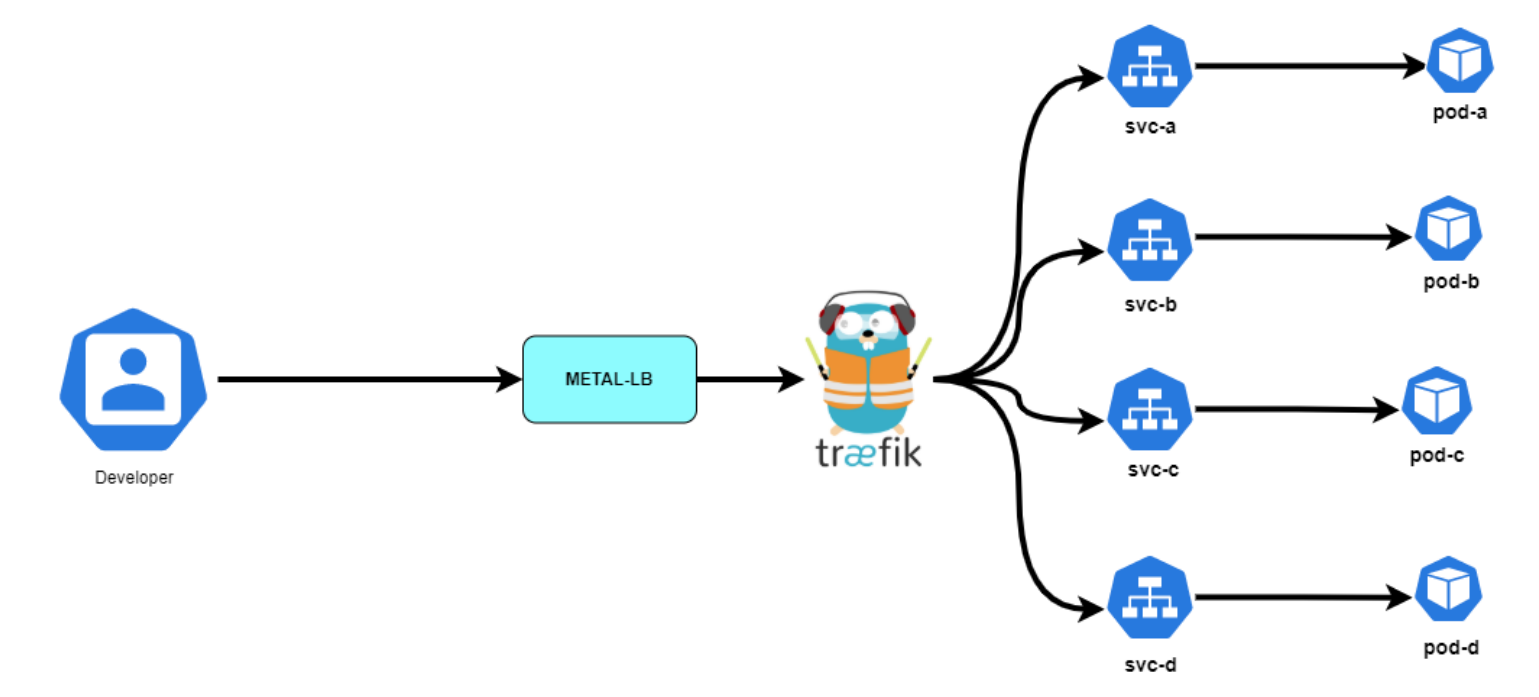
\includegraphics[width=1\textwidth]{figures/kubernetes-arch.png}
    \caption{Arsitektur Kubernetes yang akan digunakan}
\end{figure}
\newpage